\documentclass[12pt]{article}

\usepackage{fullpage}
\usepackage[round]{natbib}
\usepackage{multirow}
\usepackage{booktabs}
\usepackage{graphicx}
\usepackage{float}
\usepackage[usenames,dvipsnames]{xcolor}
\usepackage{hyperref}
\usepackage[numbib,nottoc]{tocbibind}

\hypersetup{
bookmarks=true,     % show bookmarks bar?
colorlinks=true,       % false: boxed links; true: colored links
linkcolor=red,          % color of internal links (change box color with linkbordercolor)
citecolor=blue,      % color of links to bibliography
filecolor=magenta,  % color of file links
urlcolor=cyan          % color of external links
}

%% Comments
\newif\ifcomments\commentstrue

\ifcomments
\newcommand{\authornote}[3]{\textcolor{#1}{[#3 ---#2]}}
\newcommand{\todo}[1]{\textcolor{red}{[TODO: #1]}}
\else
\newcommand{\authornote}[3]{}
\newcommand{\todo}[1]{}
\fi
\newcommand{\wss}[1]{\authornote{magenta}{SS}{#1}}
\newcommand{\nk}[1]{\authornote{blue}{NK}{#1}}

\newcounter{acnum}
\newcommand{\actheacnum}{AC\theacnum}
\newcommand{\acref}[1]{AC\ref{#1}}

\newcounter{ucnum}
\newcommand{\uctheucnum}{UC\theucnum}
\newcommand{\uref}[1]{UC\ref{#1}}

\newcounter{mnum}
\newcommand{\mthemnum}{M\themnum}
\newcommand{\mref}[1]{M\ref{#1}}

\newcommand{\progname}{GlassBR}

\begin{document}

\title{Module Guide for \progname} 
\author{Spencer Smith and Thulasi Jegatheesan}
\date{\today}
	
\maketitle

\tableofcontents

\newpage

\section{Introduction}

Decomposing a system into modules is a commonly accepted approach to developing
software.  A module is a work assignment for a programmer or programming
team~\citep{ParnasEtAl1984}.  In the best practices for scientific computing,
\citet{WilsonEtAl2013} advise a modular design, but are silent on the criteria
to use to decompose the software into modules.  We advocate a decomposition
based on the principle of information hiding~\citep{Parnas1972a}.  This
principle supports design for change, because the ``secrets'' that each module
hides represent likely future changes.  Design for change is valuable in SC,
where modifications are frequent, especially during initial development as the
solution space is explored.  

Our design follows the rules layed out by \citet{ParnasEtAl1984}, as follows:
\begin{itemize}
\item System details that are likely to change independently should be the
  secrets of separate modules.
\item Each data structure is used in only one module.
\item Any other program that requires information stored in a module's data
  structures must obtain it by calling access programs belonging to that module.
\end{itemize}

After completing the first stage of the design, which is the Software Requirements
Specification (SRS), the Module Guide (MG) is developed~\citep{ParnasEtAl1984}. 
The MG
specifies the modular structure of the system and is intended to allow both
designers and maintainers to easily identify the parts of the software.  The
potential readers of this document are as follows:

\begin{itemize}
\item New project members: This document can be a guide for a new project member
  to easily understand the overall structure and quickly find the
  relevant modules they are searching for.
\item Maintainers: The hierarchical structure of the module guide improves the
  maintainers' understanding when they need to make changes to the system. It is
  important for a maintainer to update the relevant sections of the document
  after changes have been made.
\item Designers: Once the module guide has been written, it can be used to
  check for consistency, feasibility and flexibility. Designers can verify the
  system in various ways, such as consistency among modules, feasibility of the
  decomposition, and flexibility of the design.
\end{itemize}

The rest of the document is organized as follows. Section
\ref{SecChange} lists the anticipated and unlikely changes of the software
requirements. Section \ref{SecMH} summarizes the module decomposition that
was constructed according to the likely changes. Section \ref{SecConnection}
specifies the connections between the software requirements and the
modules. Section \ref{SecMD} gives a detailed description of the
modules. Section \ref{SecTM} includes two traceability matrices. One checks
the completeness of the design against the requirements provided in the SRS. The
other shows the relation between anticipated changes and the modules. Section
\ref{SecUse} describes the use relation between modules.

\section{Anticipated and Unlikely Changes} \label{SecChange}

This section lists possible changes to the system. According to the likeliness
of the change, the possible changes are classified into two
categories. Anticipated changes are listed in Section \ref{SecAchange}, and
unlikely changes are listed in Section \ref{SecUchange}.

\subsection{Anticipated Changes} \label{SecAchange}

Anticipated changes are the source of the information that is to be hidden
inside the modules. Ideally, changing one of the anticipated changes will only
require changing the one module that hides the associated decision. The approach
adapted here is called design for
change. Anticipated changes are numbered by \textbf{AC} followed by a number.

\begin{description}

\item[\refstepcounter{acnum} \actheacnum \label{acHardware}:] The specific
  hardware on which the software is running.
\item[\refstepcounter{acnum} \actheacnum \label{acInputFormat}:] The format of the
  input parameters external to the software.
\item[\refstepcounter{acnum} \actheacnum \label{acParamsStruct}:] The data structure
  used internally to store the input parameters.
\item[\refstepcounter{acnum} \actheacnum \label{acVerific}:] Rules for
  verification of the input data.
\item[\refstepcounter{acnum} \actheacnum \label{acInASTMFormat}:] The format of the
  ASTM data tables.
\item[\refstepcounter{acnum} \actheacnum \label{acOutput}:] The format of the
  final output data.
\item[\refstepcounter{acnum} \actheacnum \label{acCalc}:] How the calculation
  equations are defined.
\item[\refstepcounter{acnum} \actheacnum \label{acControl}:] How the overall
  control of the calculations is orchestrated.
\item[\refstepcounter{acnum} \actheacnum \label{acConstants}:] The values of
  constants.
\item[\refstepcounter{acnum} \actheacnum \label{acGlassType}:] The
  implementation of the ``glass type'' type.
\item[\refstepcounter{acnum} \actheacnum \label{acThickness}:] The
  implementation of the thickness type.
\item[\refstepcounter{acnum} \actheacnum \label{acFuncts}:] The data structure
  used to represent a two dimensional function.
\item[\refstepcounter{acnum} \actheacnum \label{acContours}:] The data structure used
  to represent a sequence of two dimensional functions as contours.
\item[\refstepcounter{acnum} \actheacnum \label{acSeqServices}:] The algorithms
  used to provide typical services on a sequence of numbers, such as checking
  for ascending, interpolation, etc.

\end{description}

\subsection{Unlikely Changes} \label{SecUchange}

The module design should be as general as possible. However, generality can introduce complexity, which can, at times, be avoided by explicitly fixing some decision decisions as unlikely changes. If
these decisions should later need to be changed, then many parts of the design
will potentially need to be modified. Hence, it is not intended that these
decisions will be changed.  As an example, the equations for calculating the 
blast risk  are assumed to follow the structure given in the SRS; that is,
even if they need to be modified, the modifications should be possible by
changing how the input parameters are used in the definition.  If new parameters
are needed, this will mean a change to both the input parameters module, the
calculation module and the output module.
 Unlikely changes are numbered by \textbf{UC}
followed by a number.

\begin{description}
\item[\refstepcounter{ucnum} \uctheucnum \label{ucIO}:] Input/Output devices
  (Input: File and/or Keyboard, Output: File, Memory, and/or Screen).
\item[\refstepcounter{ucnum} \uctheucnum \label{ucInput}:] There will always be
  a source of input data external to the software.
\item[\refstepcounter{ucnum} \uctheucnum \label{ucOutput}:] Output data are
  displayed to the output device.
\item[\refstepcounter{ucnum} \uctheucnum \label{ucGoal}:] The goal of the system
  is to predict whether the glass slab under consideration can withstand an 
  explosion of a certain degree.
\item[\refstepcounter{ucnum} \uctheucnum \label{ucODEstructure}:] The 
equations for safety can be defined using parameters defined in the input parameters 
module.

\end{description}

\section{Module Hierarchy} \label{SecMH}


This section provides an overview of the module design. Modules are summarized
in a hierarchy decomposed by secrets in Table \ref{TblMH}. The modules listed
below, which are leaves in the hierarchy tree, are the modules that will
actually be implemented.  Modules are numbered by \textbf{M}
followed by a number.

\begin{description}
\item [\refstepcounter{mnum} \mthemnum \label{mHH}:] Hardware-Hiding
\item [\refstepcounter{mnum} \mthemnum \label{mParams}:] Input
\item [\refstepcounter{mnum} \mthemnum \label{mLoad}:] LoadASTM
\item [\refstepcounter{mnum} \mthemnum \label{mOutput}:] Output
\item [\refstepcounter{mnum} \mthemnum \label{mCalc}:]  Calc
\item [\refstepcounter{mnum} \mthemnum \label{mControl}:] Control
\item [\refstepcounter{mnum} \mthemnum \label{mConstants}:] Constants
\item [\refstepcounter{mnum} \mthemnum \label{mGlassType}:] GlassTypeADT
\item [\refstepcounter{mnum} \mthemnum \label{mThickness}:] ThicknessADT
\item [\refstepcounter{mnum} \mthemnum \label{mFunctADT}:] FunctADT
\item [\refstepcounter{mnum} \mthemnum \label{mContoursADT}:] ContoursADT
\item [\refstepcounter{mnum} \mthemnum \label{mSeqServices}:] SeqServices
\end{description}

Note that \mref{mHH} is a commonly used module and is already implemented by 
the operating system.  It will not be reimplemented.

\section{Connection Between Requirements and Design} \label{SecConnection}

The design of the system is intended to satisfy the requirements developed in
the SRS. In this stage, the system is decomposed into modules. The connection
between requirements and modules is listed in Table \ref{TblRT}.

\section{Module Decomposition} \label{SecMD}

Modules are decomposed according to the principle of ``information hiding''
proposed by \citet{ParnasEtAl1984}. The \emph{Secrets} field in a module
decomposition is a brief statement of the design decision hidden by the
module. The \emph{Services} field specifies \emph{what} the module will do
without documenting \emph{how} to do it. For each module, a suggestion for the
implementing software is given under the \emph{Implemented By} title. If the
entry is \emph{OS}, this means that the module is provided by the operating
system or by standard programming language libraries. If the entry is
\emph{Python}, this means that the module is provided by Python.  
\emph{\progname} means the module will be implemented by the \progname{} software.  
% should reference a command for the name, in case it changes
Only the leaf modules in the
hierarchy have to be implemented. If a dash (\emph{--}) is shown, this means
that the module is not a leaf and will not have to be implemented. Whether or
not this module is implemented depends on the programming language
selected.

\begin{table}[h!]
\centering
\begin{tabular}{p{0.3\textwidth} p{0.6\textwidth}}
\toprule
\textbf{Level 1} & \textbf{Level 2}\\
\midrule

{Hardware-Hiding} & ~ \\
\midrule

\multirow{8}{0.3\textwidth}{Behaviour-Hiding Module} 
& Input\\
& LoadASTM\\
& Output\\
& Calc\\
& Control\\
& GlassTypeADT\\
& ThicknessADT\\
& Constants\\

\midrule

\multirow{1}{0.3\textwidth}{Software Decision}
& FunctADT\\
& ContoursADT\\
& SeqServices\\

\bottomrule

\end{tabular}
\caption{Module Hierarchy}
\label{TblMH}
\end{table}

\subsection{Hardware Hiding Modules (\mref{mHH})}

\begin{description}
\item[Secrets:]The data structure and algorithm used to implement the virtual
  hardware.
\item[Services:]Serves as a virtual hardware used by the rest of the
  system. This module provides the interface between the hardware and the
  software. So, the system can use it to display outputs or to accept inputs.
\item[Implemented By:] OS
\end{description}

\subsection{Behaviour-Hiding Module}

\begin{description}
\item[Secrets:]The contents of the required behaviours.
\item[Services:]Includes programs that provide externally visible behaviour of
  the system as specified in the software requirements specification (SRS)
  documents. This module serves as a communication layer between the
  hardware-hiding module and the software decision module. The programs in this
  module will need to change if there are changes in the SRS.
\item[Implemented By:] --
\end{description}

\subsubsection{Input (\mref{mParams})}

\begin{description}
\item[Secrets:] The data structure for input parameters, how the
values are input and how the values are verified.  The load and verify secrets
are isolated to their own access programs (like submodules).  This, combined
with the fact that all of the services are invoked together, suggests that the
one module one secret rule can be relaxed in this instance.
\item[Services:] Gets input from user, stores input and verifies that the
  input parameters comply with physical and software constraints. Throws an
  error if a parameter violates a physical constraint. Throws a warning if a
  parameter violates a software constraint.  Stored parameters can be read
  individually, but write access is only to redefine the entire set of inputs.
\item[Implemented By:] \progname{}
\end{description}

\subsubsection{LoadASTM (\mref{mLoad})}

\begin{description}
\item[Secrets:] The format of the two ASTM data tables: i) 3 second equivalent
  pressure ($q$) versus stand off distance (SD) versus charge weight ($w$), and
  ii) Non dimensional lateral load ($\hat q$) versus aspect ration versus Stress
  distribution factor ($J$).
\item[Services:] Reads the data from each ASTM file and creates an object that
  stores the sequence of functions represented by the data for each table of
  data.
\item[Implemented By:] \progname{}
\end{description}

\subsubsection{Output Module (\mref{mOutput})}

\begin{description}
\item[Secrets:] The format and structure of the output data.
\item[Services:] Outputs the results of the calculations, including the input
  parameters, the demand, the capacity, the probability of breakage, and both 
  safety requirements.
\item[Implemented By:] \progname{}
\end{description} 

\subsubsection{Calc Module (\mref{mCalc})}

\begin{description}
\item[Secrets:] The equations for predicting the probability of glass 
breakage, capacity, and demand, using the input parameters.
\item[Services:] Defines the equations for solving for the probability of glass 
breakage, demand, and capacity using the parameters in the input parameters 
module.
\item[Implemented By:] \progname{}
\end{description} 
 
\subsubsection{Control Module (\mref{mControl})}

\begin{description}
\item[Secrets:] The algorithm for coordinating the running of the program.
\item[Services:] Provides the main program.
\item[Implemented By:] \progname{}
\end{description}

\subsubsection{Constants Module (\mref{mConstants})}

\begin{description}
\item[Secrets:] The values of constants and new types.
\item[Services:] Provides constants and types used by other modules.
\item[Implemented By:] \progname{}
\end{description}

\subsubsection{GlassTypeADT Module (\mref{mGlassType})}

\begin{description}
\item[Secrets:] The implementation of the ``glass type'' type.
\item[Services:] Defines abstract data type for glass type.
\item[Implemented By:] \progname{}
\end{description}

\subsubsection{ThicknessADT Module (\mref{mThickness})}

\begin{description}
\item[Secrets:] The implementation of the thickness type.
\item[Services:]  Defines abstract data type for thickness.
\item[Implemented By:] \progname{}
\end{description}

\subsection{Software Decision Module}

\begin{description}
\item[Secrets:] The design decision based on mathematical theorems, physical
  facts, or programming considerations. The secrets of this module are
  \emph{not} described in the SRS.
\item[Services:] Includes data structure and algorithms used in the system that
  do not provide direct interaction with the user. 
  % Changes in these modules are more likely to be motivated by a desire to
  % improve performance than by externally imposed changes.
\item[Implemented By:] --
\end{description}

\subsubsection{FunctADT Module (\mref{mFunctADT})}

\begin{description}
\item[Secrets:] The data structure used to represent a two dimensional
  function.  For instance, the data may be represented by a table of data, or a
  polynomial, or a piecewise linear function, etc.
\item[Services:] Defines the abstract data type for functions, providing a
  constructor and a means to evaluate the function for a given value of the
  independent variable.
\item[Implemented By:] \progname{}
\end{description}

\subsubsection{ContoursADT Module (\mref{mContoursADT})}

\begin{description}
\item[Secrets:] The data structure used to represent a
  sequence of two dimensional functions in the form of contours.  Each function
  is associated with a particular value, like a contour in a contour map.
\item[Services:] Defines the abstract data type for a sequence of functions.
  Allows adding/removing functions to/from the sequence.  Provides evaluation of
  the 3d function at values between the contours.
\item[Implemented By:] \progname{}
\end{description}

\subsubsection{SeqServices Module (\mref{mSeqServices})}

\begin{description}
\item[Secrets:] The algorithms for services related to sequences of numbers.
\item[Services:] Provides functions operating on sequences of numbers, such as
  checks for monotonically increasing values and interpolation.
\item[Implemented By:] \progname{}
\end{description}

\section{Traceability Matrix} \label{SecTM}

This section shows two traceability matrices: between the modules and the
requirements and between the modules and the anticipated changes.  We should
also consider documenting the mapping between these ``abstract'' modules and the
Python files.

% the table should use mref, the requirements should be named, use something
% like fref
\begin{table}[H]
\centering
\begin{tabular}{p{0.2\textwidth} p{0.6\textwidth}}
  \toprule
  \textbf{Req.} & \textbf{Modules}\\
  \midrule
  R1 & \mref{mHH}, \mref{mParams}, \mref{mControl}\\
  R2 & \mref{mParams}, \mref{mGlassType}, \mref{mThickness}\\
  R3 & \mref{mParams}, \mref{mConstants}\\
  R4 & \mref{mOutput}, \mref{mGlassType}, \mref{mThickness}\\
  R5 & \mref{mLoad}, \mref{mOutput}, \mref{mCalc}, \mref{mConstants}, \mref{mFunctADT},
       \mref{mContoursADT}, \mref{mSeqServices}\\
  R6 & \mref{mOutput}\\
  \bottomrule
\end{tabular}
\caption{Trace Between Requirements and Modules}
\label{TblRT}
\end{table}

\begin{table}[H]
\centering
\begin{tabular}{p{0.2\textwidth} p{0.6\textwidth}}
\toprule
\textbf{AC} & \textbf{Modules}\\
\midrule
\acref{acHardware} & \mref{mHH}\\
\acref{acInputFormat} & \mref{mParams}\\
\acref{acParamsStruct} & \mref{mParams}\\
\acref{acVerific} & \mref{mParams}\\
\acref{acInASTMFormat} & \mref{mLoad}\\
\acref{acOutput} & \mref{mOutput}\\
\acref{acCalc} & \mref{mCalc}\\
\acref{acControl} & \mref{mControl}\\
\acref{acConstants} & \mref{mConstants}\\
\acref{acGlassType} & \mref{mGlassType}\\
\acref{acThickness} & \mref{mThickness}\\
\acref{acFuncts} & \mref{mFunctADT}\\
\acref{acContours} & \mref{mContoursADT}\\
\acref{acSeqServices} & \mref{mSeqServices}\\
\bottomrule
\end{tabular}
\caption{Trace Between Anticipated Changes and Modules}
\label{TblAC}
\end{table}
\section{Use Hierarchy Between Modules} \label{SecUse}

In this section, the uses hierarchy between modules is
provided. \citet{Parnas1978} said of two programs A and B that A {\em uses} B if
correct execution of B may be necessary for A to complete the task described in
its specification. That is, A {\em uses} B if there exist situations in which
the correct functioning of A depends upon the availability of a correct
implementation of B.  Figure \ref{FigUH} illustrates the use relation between
the modules. It can be seen that the graph is a directed acyclic graph
(DAG). Each level of the hierarchy offers a testable and usable subset of the
system, and modules in the higher level of the hierarchy are essentially simpler
because they use modules from the lower levels.

\begin{figure}[H]
	\centering
	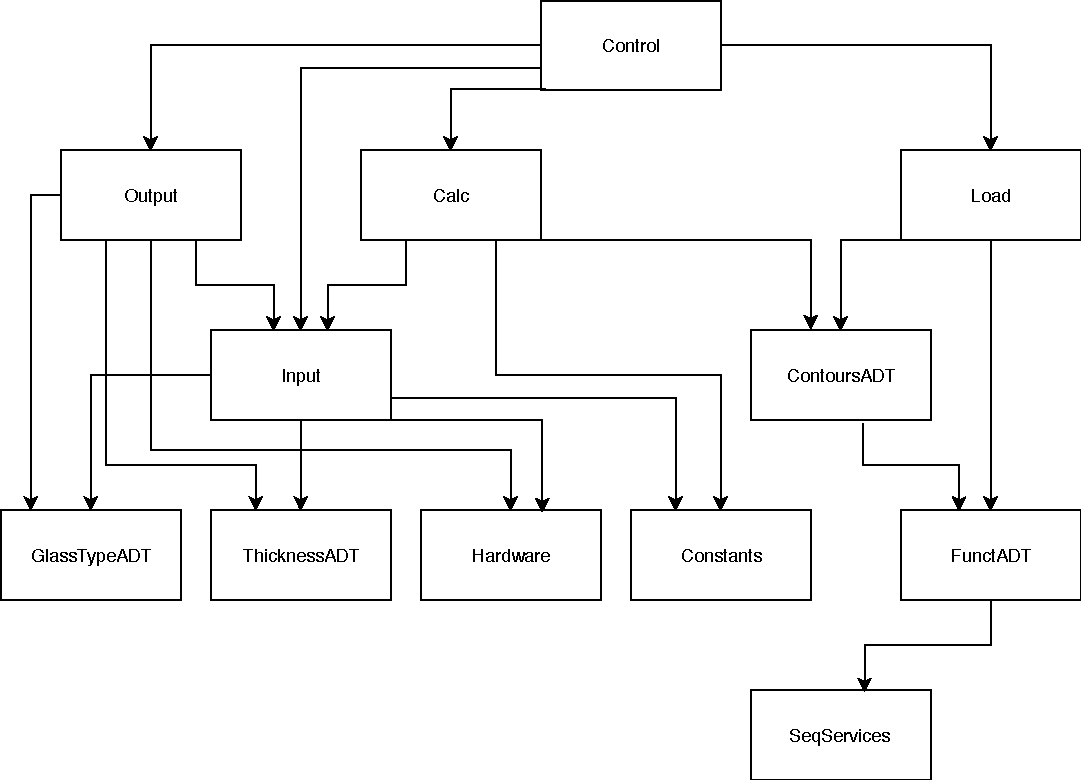
\includegraphics[width=0.7\textwidth]{GlassBR-UsesHierarchy.pdf}
	\caption{Use Hierarchy among Modules}
	\label{FigUH}
\end{figure}

%\section*{References}

\bibliographystyle {plainnat}
\bibliography {../../../refs/References}

\end{document}
